\documentclass[11pt, a4paper, spanish]{article}

%%%%%%%%%% COMIENZO DEL PREAMBULO %%%%%%%%%%

%Info sobre este documento
\author{Martin Cammi}
\title{Trabajo Pr'actico de Ingenier'ia del software I}

%\usepackage{infostyle}                                                  % provee un look & feel similar a un documento Word
\usepackage[top=2.5cm, bottom=2.5cm, left=2.5cm, right=2.5cm]{geometry}  % m\'argenes
\usepackage[ansinew]{inputenc}                                           % permite que los acentos del estilo \'a\'e\'i\'o\'u salgan joya
\usepackage[spanish, activeacute]{babel}                                 % idioma espa\~{n}ol, acentos f\'aciles y deletreo de palabras
\usepackage{indentfirst}                                                 % permite indentar un parrafo a mano
\usepackage{caratula}                                                    % incluye caratula est\'andar
\usepackage{graphicx}                                                    % permite insertar gr\'aficos
\usepackage{color}                                                       % permite el uso de colores en el documento
\usepackage[pdfcreator={TexLive!, LaTeX2e con TeXnicCenter;-)},
			pdfauthor={Grupo 2"},
			pdftitle={Base de Datos - Trabajo practico:},
			pdfsubject={Trabajo Practico de Buffer Manager},
			pdfkeywords={MER, MR},
			pdfstartview=FitH,            % Fits the width of the page to the window
			bookmarksnumbered,            % los bookmarks numerados se ven mejor...
			colorlinks,                   % links con bellos colores
			linkcolor=magenta]            % permite cambiar el color de los links
			{hyperref}                    % Permite jugar con algunas cosas que aparecer\'an en el PDF final
\usepackage{hyperref}
\usepackage{rotating}
\usepackage{ulem}
\usepackage[dash]{dashundergaps}
\usepackage{multicol}


%\selectlanguage{spanish}

\linespread{1.3}                    % interlineado equivalente al 1.5 l\'ineas de Word...
\pagestyle{myheadings}              %encabezado personalizable con \markboth{}{}
\markboth{}{Trabajo pr\'actico 2 (Cammi, De Sousa) }
\headsep = 30pt                     % separaci\'on entre encabezado y comienzo del p\'arrafo

%\addtolength{\oddsidemargin}{-2cm}	% configuracion IDEAL!!!
%\addtolength{\textwidth}{4cm}
%\addtolength{\textheight}{2cm}

% macro 'todo' para To-Do's
\def\todo#1{\textcolor{red}{#1}}

% Macro 'borde' para un texto con borde
\newsavebox{\fmbox}
\newenvironment{borde}[1]
{\begin{lrbox}{\fmbox}\begin{minipage}{#1}}
{\end{minipage}\end{lrbox}\fbox{\usebox{\fmbox}}\\[10pt]}

%%%%%%%%%% FIN DEL PREAMBULO %%%%%%%%%%

\begin{document}

\materia{Base de Datos}
\submateria{Segundo Cuatrimestre de 2012}
\titulo{Trabajo pr\'actico 2}
\subtitulo{Buffer Manager y estrategias de reemplazo de p'aginas}
\grupo{Grupo 2}

\integrante{Cammi, Mart\'in}{676/02}{martincammi@gmail.com}
\integrante{De Sousa, Mariano}{389/08}{marian\_sabianaa@hotmail.com}

\maketitle

\thispagestyle{empty}

\tableofcontents

\newpage

% Conviene poner las secciones como diferentes archivos,
% sobre todo cuando se trabaja en equipo.
% Es m\'as f\'acil para sincronizar mediante control de versiones.
%\input{Introducci\'on}


% BEGIN Ejemplos de uso

	%\section{Una secci\'on}
	%\label{sec:unaSeccion}
	%Hola! Soy una Secci\'on
	%	\subsection{Una subsecci\'on}
	%		Y yo soy una subsecci\'on!!!
	%		\subsubsection{Una subsubsecci\'on}
	%			Y yo soy una sub-subsecci\'on!!!
	%			\paragraph{Un p\'arrafo\\}
	%				Y yo soy un p\'arrafo, porque no hay mas sub-sub-sub-subsecciones!!!

	%\section{Otra secci\'on}
	%	Como pudimos ver en la secci\'on \ref{sec:unaSeccion}, esto es una demo de una referencia a una secci\'on.
	
	%	Tambi\'en podemos hacer referencia a la p\'agina de la secci\'on:\\[10pt]
	
		% Ejemplo de uso de un borde (falta pulir para que no tire un warning!)
	%	\begin{borde}{0.98\textwidth}
	%		En la p\'agina \pageref{sec:unaSeccion}, hay una secci\'on pilla...
	%	\end{borde}

% END Ejemplos de uso

\newpage 
\section{Investigaci'on sobre estrategia de reemplazo de p'aginas de Oracle}

\subsection{Introducci\'on}

A lo largo de este trabajo analizaremos el algoritmo de \textit{Touch Count} dise\~{n}ado por \textit{Oracle} para administrar en memoria las p\'aginas que se
traen de la base de datos con el objetivo de evitar los accesos a disco y por consiguiente, obtener mejor\'ia en el rendimiento del motor.\\

Inicialmente Oracle utilizaba para el algoritmo de manejo de \textit{cach\'e} lo que se conoce como algoritmo LRU (Least Recently Used). Este algoritmo, 
descripto m\'as adelante se basa en priorizar en la cach\'e las p\'aginas de disco m\'as referenciadas descartando las menos usadas recientemente 
(definici\'on de LRU).\\

Un caso muy com\'un que presenta un problema a este algoritmo son los full scan, los cuales recorren todos los registros de una tabla coloc\'andolos en 
la \textit{cach'e} y pisando todo historial previo. As\'i por ejemplo, si la cache del buffer tiene 300 bloques y un escaneo completo de una 
tabla est'a recibiendo 400 bloques en la cache del buffer, todos los bloques populares desaparecer'an. \\

Para superar este problema, Oracle propuso un algoritmo modificado de LRU al que denomin\'o \textit{Touch Count}
  
\subsection{Algoritmo \textit{Touch Count}}

El algoritmo \textit{Touch Count} utiliza las idea de los algoritmos de LRU y MRU. Prioriza mantener en la cach\'e las p\'aginas m\'as referenciadas y descartar las menos, manteniendo una lista LRU y reorden\'andola con un criterio que se asemeja con el desalojo de MRU: quien sea el m\'as referenciado se reubicar'a, para ello el algoritmo llevar\'a un conteo de cuantas veces fue referenciada. Este n\'umero
de referencias a la p\'agina se denomina \textit{Touch Count}.

\subsection{Problem\'atica que resuelve}

Uno de los problemas que el \textit{Touch Count} resuelve es el de las r\'afagas de acceso a p\'aginas. En un full scan por ejemplo m\'ultiples p\'aginas
son referenciadas las que potencialmente pueden borrar la cach\'e. Que una p\'agina sea referenciada espor\'adicamente no implica que permanecer\'a en memoria, deber\'a volver a pedirla, que aumente su \textit{Touch Count} para as\'i poder alejarse de la zona fr\'ia donde es m\'as propensa a ser desalojada.

\newpage 
\section{Implementaci'on estrategias de reemplazo de p'aginas}

\subsection{Algoritmo de LRU}

El algoritmo LRU (Least Recently Used) funciona de la siguiente manera, mantiente en memoria las p\'aginas m\'as recientemente usadas
y en caso de necesitar remover alguna, elige la que se posee fecha de referencia m\'as vieja.\\

El siguiente es un ejemplo de como la cach\'e se va actualizando mediante el algoritmo LRU.\\

El gr\'afico a continuaci\'on se lee de izquierda a derecha de arriba abajo. La primera hilera de n\'umeros corresponde a la traza de p\'aginas que intentan ser 
accedidas. Debajo de ella aparece en forma vertical la cach\'e y como se va llenando a medida que c\'ada p\'agina de la traza es referenciada.\\ 

Marcaremos con amarillo cuando ocurra un \textit{Hit} y con gris cuando ocurra un \textit{Miss}.
Cuando una p\'agina sea referenciada la marcaremos en la cach\'e en negrita para saber que fue la m\'as recientemente accedida.\\

\begin{center}
		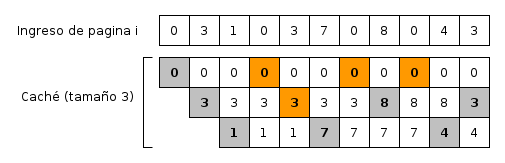
\includegraphics[scale=0.65]{diagramas/LRUAlgorithm.png}\\
\end{center}

As\'i en el ejemplo, 
\begin{itemize}
	\item{ Se referencia inicialmente la p\'agina 0, como la cach\'e se encuentra vac\'ia se produce un \textit{Miss}, y se prodece a agregar
		la p\'agina 0 a la cach\'e.}
	\item{ Se referencia a la p\'agina 3, como no existe en la cach\'e (ya que solo posee la p\'agina 0 agregada anterioremente) se produce 
		un \textit{Miss} y se prodece a agregar la p\'agina 3 a la cach\'e.}
	\item{ Se referencia a la p\'agina 1, como no existe en la cach\'e se produce un \textit{Miss} y se prodece a agregar la p\'agina 1 a la cach\'e.}
	\item{ Se referencia a la p\'agina 0, como existe en la cach\'e se produce un \textit{Hit}. }
	\item{ Se referencia a la p\'agina 3, como existe en la cach\'e se produce un \textit{Hit}. }
	\item{ Se referencia a la p\'agina 7, como no existe en la cach\'e se produce un \textit{Miss} y se prodece a agregar la p\'agina 7 a la cach\'e
		reemplazando la menos recientemente usada que es la p\'agina 1. }
	\item{ Se referencia a la p\'agina 0, como existe en la cach\'e se produce un \textit{Hit}. }
	\item{ Se referencia a la p\'agina 8, como no existe en la cach\'e se produce un \textit{Miss} y se prodece a agregar la p\'agina 8 a la cach\'e
		reemplazando la menos recientemente usada que es la p\'agina 3. }
	\item{ Se referencia a la p\'agina 0, como existe en la cach\'e se produce un \textit{Hit}. }
	\item{ Se referencia a la p\'agina 4, como no existe en la cach\'e se produce un \textit{Miss} y se prodece a agregar la p\'agina 4 a la cach\'e
		reemplazando la menos recientemente usada que es la p\'agina 7. }
	\item{ Se referencia a la p\'agina 3, como no existe en la cach\'e (porque ya fue desalojada) se produce un \textit{Miss} y se prodece a agregar 
		la p\'agina 3 a la cach\'e reemplazando la menos recientemente usada que es la p\'agina 8. }
\end{itemize}

Es interesante notar que una p\'agina no ser\'a desalojada hasta tanto se hayan referenciado al menos una vez a todas las otras, ya que de esta forma
la p\'agina inicial se convertir\'ia en la menos recientemente usada.\\

\noindent{\emph{Cantidad de Hits:} 4} \\
\emph{Cantidad de Miss:} 7, con un total de 3 \emph{Miss} iniciales y 4 \emph{Miss} a lo largo de la traza.\\
\emph{Predicci\'on:} Este enfoque se basa en el principio de vecindad temporal; p\'aginas que fueron referenciadas posiblemente lo sean en un per\'iodo corto de tiempo.\\
\emph{Desventajas:} Una desventaja es que una consulta que traiga muchas p\'aginas que no vuelvan a ser utilizadas (ej: full scan sobre una tabla), barrer\'a gran parte, sino toda, las entradas existentes en la cach\'e.\\
\emph{Ventajas:} En un contexto donde el principio de vecindad temporal es v\'alido, mientras un conjunto de p\'aginas se referencie con 
periocidad (en ventanas cortas de tiempo), existe una alta probabilidad que la p\'agina se encuentre en memoria.\\

\newpage
\subsection{Algoritmo de MRU}

El algoritmo MRU (Most Recently Used) funciona a la inversa de \textit{LRU}, intentando mantener en memoria las p\'aginas menos recientemente usadas
y en caso de necesitar remover alguna eligiendo de entre alguna de las m\'as recientemente usadas.\\

El siguiente es un ejemplo de como las cach\'e se va actualizando mediante el algoritmo LRU.\\

El gr\'afico a continuaci\'on se lee de izquierda a derecha de arriba abajo. La primera hilera de n\'umeros corresponde a la traza de p\'aginas que intentan ser 
accedidas. Debajo de ella aparece en forma vertical la cach\'e y como se va llenando a medida que c\'ada p\'agina de la traza es referenciada.\\ 

Marcaremos con amarillo cuando ocurra un \textit{Hit} y con gris cuando ocurra un \textit{Miss}.
Cuando una p\'agina sea referenciada la marcaremos en la cach\'e en negrita para saber que fue la m\'as recientemente accedida.\\

\begin{center}
		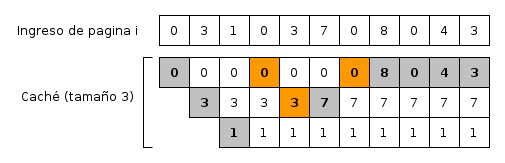
\includegraphics[scale=0.65]{diagramas/MRUAlgorithm.png}\\
\end{center}



As\'i en el ejemplo, 

\begin{itemize}
	\item{ Se referencia inicialmente la p\'agina 0, como la cach\'e se encuentra vac\'ia se produce un \textit{Miss}, y se prodece a agregar
		la p\'agina 0 a la cach\'e.}
	\item{ Se referencia a la p\'agina 3, como no existe en la cach\'e (ya que solo posee la p\'agina 0 agregada anterioremente) se produce 
		un \textit{Miss} y se prodece a agregar la p\'agina 3 a la cach\'e.}
	\item{ Se referencia a la p\'agina 1, como no existe en la cach\'e se produce un \textit{Miss} y se prodece a agregar la p\'agina 1 a la cach\'e.}
	\item{ Se referencia a la p\'agina 0, como existe en la cach\'e se produce un \textit{Hit}. }
	\item{ Se referencia a la p\'agina 3, como existe en la cach\'e se produce un \textit{Hit}. }
	\item{ Se referencia a la p\'agina 7, como no existe en la cach\'e se produce un \textit{Miss} y se prodece a agregar la p\'agina 7 a la cach\'e
		reemplazando la m\'as recientemente usada que es la p\'agina 3. }
	\item{ Se referencia a la p\'agina 0, como existe en la cach\'e se produce un \textit{Hit}. }
	\item{ Se referencia a la p\'agina 8, como no existe en la cach\'e se produce un \textit{Miss} y se prodece a agregar la p\'agina 8 a la cach\'e
		reemplazando la m\'as recientemente usada que es la p\'agina 0. }
	\item{ Se referencia a la p\'agina 0, como no existe en la cach\'e (porque ya fue desalojada) se produce un \textit{Miss} y se prodece a agregar 
		la p\'agina 0 a la cach\'e reemplazando la m\'as recientemente usada que es la p\'agina 8. }
	\item{ Se referencia a la p\'agina 4, como no existe en la cach\'e se produce un \textit{Miss} y se prodece a agregar 
		la p\'agina 4 a la cach\'e reemplazando la m\'as recientemente usada que es la p\'agina 0. }
	\item{ Se referencia a la p\'agina 3, como no existe en la cach\'e (porque ya fue desalojada) se produce un \textit{Miss} y se prodece a agregar 
		la p\'agina 3 a la cach\'e reemplazando la m\'as recientemente usada que es la p\'agina 4. }
\end{itemize}

En este algoritmo se puede notar que cualquier referencia a una p\'agina existente en la cach\'e la convierte en la potencial primera v\'ictima 
para ser desalojada en caso de un pr\'oximo \textit{Miss}.\\

\noindent{\emph{Cantidad de Hits:} 3}\\
\emph{Cantidad de Miss:} 8, con un total de 3 \textit{Miss} iniciales y 5 \textit{Miss} a lo largo de la traza. \\
\emph{Predicci\'on:} Este tipo de enfoque intenta basarse en que una vez referenciada una p\'agina no volver\'a a serlo al menos en un cierto per\'iodo
de tiempo en el cual si podr\'ian llegar a serlo p\'aginas m\'as antiguas.\\
\emph{Desventajas:} Si la cach\'e se encuentra llena con p\'aginas que no ser\'an referenciadas en un tiempo cercano y se consultan nuevas, deber'a continuamente estar desalojando una p\'agina para poder agregarlas (notar que en cada r\'afaga s\'olo quedar\'a la \'ultima de ellas).\\
\emph{Ventajas:} Las p\'aginas que se consultan de manera espor\'adica ser\'an r\'apidamente desalojadas sin afectar al resto de la cach\'e.\\

\newpage
\subsection{Algoritmo de Touch Count}

Este algoritmo es la mejora del LRU implementada por \textit{Oracle}. A continuaci\'on describiremos un poco de la estructura interna que utiliza el \textit{Touch Count}.\\

El algoritmo Touch Count cuenta con tres elementos principales: una lista, un puntero, y un contador de referencias denominado \textit{Touch Count}. 
La lista se utilizar\'a para manejar las p\'aginas y las prioridades que se le asignar\'an a cada
una esta lista estar\'a dividida en dos \'areas o regiones. La regi\'on de la izquierda de la lista denominada \textit{regi\'on fria} y la regi\'on inmediata
contigua denominada \textit{regi\'on caliente}.\\

Ambas regiones estar\'an separadas por un puntero, al que llamaremos midPointer, que se encargar\'a de marcar dicha divisi\'on. 
En realidad en la implementaci\'on el \textit{midpointer} estar\'a apuntando el primer elemento de la \textit{regi\'on caliente} cuando haya
elementos en dicha regi\'on o al final de la lista en caso contrario.\\

Por otro lado el algoritmo es configurable y cuenta con varios par\'ametros:

\begin{center}
	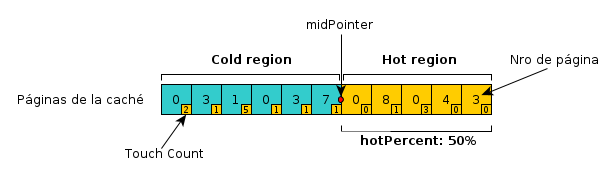
\includegraphics[scale=0.65]{diagramas/TouchCountAlgorithm1.png}\\
\end{center}

\begin{itemize}
	\item{\emph{hotPercent}: Indica el porcentaje de p\'aginas que se quieren mantener en la \textit{regi\'on caliente}. Si el porcentaje no
da exacto se toma la cantidad de p\'aginas que conformen el porcentaje inmediato inferior. }
	\item{\emph{agingTouchTime}: Es la cantidad m\'inima de tiempo a esperar antes de aumentar el \textit{touch count}  de una p\'agina ante otra referencia.}
	\item{\emph{agingWhenMoveToHot}: Es el valor al cual se establece al \textit{touch count} de una p\'agina cuando \'esta pasa a la \textit{regi\'on caliente.} }
	\item{\emph{agingToHotCriteria}: Es el valor minimo de Touch Count que debe tener una p\'agina para que pueda ser enviada a la \textit{regi\'on caliente.}}
	\item{\emph{agingCoolCount}: Es el valor de \textit{touch count} que pasa a tener la p\'agina cuando se mueve de la zona caliente a la fr\'ia.}
\end{itemize}

Ahora describiremos su comportamiento en base a las operaciones que se realizan sobre la cach\'e.

\begin{center}
	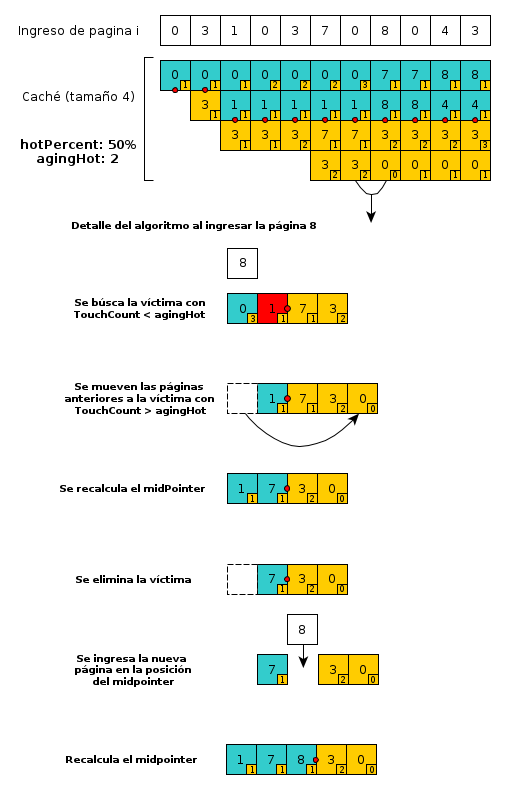
\includegraphics[scale=0.65]{diagramas/TouchCountAlgorithm2.png}\\
\end{center}

Como puede verse en el ejemplo anterior, las operaciones de \textit{agregar}, \textit{encontrar v\'ictima} y \textit{remover} hacen algunas extras que lo que indican a simple vista.

\begin{itemize}
	\item{Agregar una p\'agina:
		Si la cach\'e todav\'ia posee espacio disponible agregar\'a la nueva p\'agina en la posici\'on que indique el \textit{midPointer}.
		Si la cach\'e no posee espacio disponible proceder\'a a buscar una v\'ictima para removerla y agregar la nueva en la posici\'on del \textit{midPointer}.
	}
	\item{Encontrar v\'ictima: }
		El algoritmo comienza buscando una v\'ictima que ser\'a la primera de la regi\'on fr\'ia que tenga Touch Count menor al \textit{agingToHotCriteria}
		Una vez encontrada la v\'ictima, mover\'a todas las p\'aginas que al recorrer hayan superado el  \textit{agingToHotCriteria} al
		final de la \textit{regi\'on caliente} asign\'andole un Touch Count de \textit{agingWhenMoveToHot}. Al mismo tiempo por movimiento de estos otra p\'agina pasar\'a
		el umbral de la caliente a la fr\'ia como ocurre con la p\'agina 7 del ejemplo anterior al moverse la p\'agina 0 de la \textit{regi\'on fria}
		a la \textit{regi\'on caliente}. A estas p\'aginas que pasan a la \textit{regi\'on fria} se les colocar\'a un touch count de \textit{agingCoolCount}.
		
	\item{Remover una p\'agina: }
		El remover una p\'agina borrar\'a la p\'agina de la cach\'e y recalcular\'a la posici\'on del \textit{midpointer}.
\end{itemize}

Existe un caso particular sobre qu\'e p\'agina remover; cuando todas ellas poseen un Touch Count mayor o igual a \textit{agingToHotCriteria}. La informaci\'on recolectada no especifica qu\'e desici\'on tomar. Se opt\'o por buscar la p\'agina con Touch Count menor y en caso de existir m\'as de una, seleccionar la de fecha de referencia m\'as vieja.\\

Por otro lado, si se referencian set de datos diferentes cada vez, las p\'aginas no alcanzar\'an el valor agingToHotCriteria suficiente para salvarse en el zona caliente. De esta manera, la zona fr\'ia se comportar\'a como una LRU y las p\'aginas que queden, por el corrimiento del mid point maker, en la zona caliente; no ser\'an utilizadas desperdiciando as\'i espacio de memoria.\\

\newpage
\section{Test de Unidad}

\subsection{MRUReplacementStrategyTest}

\subsubsection{findVictim tests}

\noindent{\textbf{testNoPageToReplace:} testea que no puede obtenerse una v\'ictima porque todas las p\'aginas est\'an bloqueadas.}\\
\textbf{resultado esperado:} lanzar una PageReplacementStrategyException indicando: \textit{No page can be removed from pool}.\\

\noindent{\textbf{testOnlyOneToReplace:} testea con una \'unica p\'agina no bloqueada.}\\
\textbf{resultado esperado:} devolver la p\'agina no bloqueada como v\'ictima.\\

\noindent{\textbf{testMultiplePagesToReplace: } testea con todas p\'aginas no bloqueadas y no referenciadas.}\\
\textbf{resultado esperado:} devolver la primera como v\'ictima.\\

\noindent{\textbf{testMultiplePagesToReplaceButOldestOnePinned:}} testea con todas p\'aginas no bloqueadas salvo la \'ultima.\\
\textbf{resultado esperado:} devolver la segunda como v\'ictima.\\

\noindent{\textbf{testMultiplePagesToReplaceWithPinAndUnpin:} testea con todas las p\'aginas no bloqueadas habi\'endoselas hecho pin y unpin a cada una.}  \\
\textbf{resultado esperado:} devolver la \'ultima como v\'ictima.\\

\noindent{\textbf{testMultiplePagesToReplaceWithPinAndUnpinButOneDouble: } testea con todas las p\'aginas no bloqueadas habi\'endoselas hecho pin y unpin,
siendo que la segunda se le hizo un pin unpin m\'as.} \\
\textbf{resultado esperado:} devolver la segunda p\'agina como v\'ictima.\\ 

\noindent{\textbf{testMultiplePagesToReplaceButNewestOnePinnedWithPin: } testea con todas las p\'aginas no bloqueadas habi\'endoselas hecho pin y unpin a cada una
salvo la \'ultima a la que s\'olo se le hizo pin al final.}\\
\textbf{resultado esperado:} devolver la ante \'ultima p\'agina como v\'ictima. \\

\noindent{\textbf{testMultiplePagesToReplaceButOldestOnePinnedWithPin: } testea con todas las p\'aginas no bloqueadas habi\'endoselas hecho pin y unpin a cada una
salvo la primera a la que s\'olo se le hizo pin al final.}\\
\textbf{resultado esperado:} devolver la segunda p\'agina como v\'ictima. \\


\subsection{LRUReplacementStrategyTest}

\subsubsection{findVictim tests}

\noindent{\textbf{testNoPageToReplace:} testea que no puede obtenerse una v\'ictima porque todas las p\'aginas est\'an bloqueadas.}\\
\textbf{resultado esperado:} lanzar una PageReplacementStrategyException indicando que \textit{No page can be removed from pool}.\\

\noindent{\textbf{testOnlyOneToReplace:} testea con una \'unica p\'agina no bloqueada.}\\
\textbf{resultado esperado:} devolver la p\'agina no bloqueada como v\'ictima.\\

\noindent{\textbf{testMultiplePagesToReplace: } testea con todas p\'aginas no bloqueadas y no referenciadas.}\\
\textbf{resultado esperado:} devolver la primera como v\'ictima.\\

\noindent{\textbf{testMultiplePagesToReplaceButOldestOnePinned:}} testea con todas p\'aginas no bloqueadas salvo la \'ultima.\\
\textbf{resultado esperado:} devolver la primera como v\'ictima.\\

\noindent{\textbf{testMultiplePagesToReplaceWithPinAndUnpin:} testea con todas las p\'aginas no bloqueadas habi\'endoselas hecho pin y unpin a cada una.}  \\
\textbf{resultado esperado:} devolver la primera como v\'ictima.\\

\noindent{\textbf{testMultiplePagesToReplaceWithPinAndUnpinFirstReferencedLast: } testea con todas las p\'aginas no bloqueadas habi\'endoselas hecho pin y unpin a cada una
siendo la primera referenciada \'ultima.} \\
\textbf{resultado esperado:} devolver la segunda p\'agina como v\'ictima.\\ 

\noindent{\textbf{testMultiplePagesToReplaceButOldestOnePinnedWithPinAndUnpin: } testea con todas las p\'aginas no bloqueadas habi\'endoselas hecho pin y unpin a cada una
salvo la primera a la que s\'olo se le hizo pin al principio.}\\
\textbf{resultado esperado:} devolver la segunda p\'agina como v\'ictima. \\

\noindent{\textbf{testMultiplePagesToReplaceButOldestOnePinnedWithPinAndUnpinFirstReferencesLast: } testea con todas las p\'aginas no bloqueadas habi\'endoselas hecho pin y unpin a cada una salvo la primera a la que s\'olo se le hizo pin al final.}\\
\textbf{resultado esperado:} devolver la segunda p\'agina como v\'ictima. \\

\subsection{TouchCountBufferPoolTest}

\subsubsection{\textit{Touch Count} tests}

\noindent{\textbf{testFindVictimWithSpace:} testea la b\'usqueda de v\'ictima con espacio en la cach\'e.}\\
\textbf{resultado esperado:} lanzar una BufferPoolException indicando: \textit{The buffer still has space}. \\

\noindent{\textbf{testFindVictimWithExistingPage:} testea pasando como par\'ametro una p\'agina a agregar existente en la cach\'e.}\\
\textbf{resultado esperado:} lanzar una BufferPoolException indicando: \textit{The page is already in the buffer}. \\

\noindent{\textbf{testFindVictimInOrder:} testea con todas p\'aginas no bloqueadas.}\\
\textbf{resultado esperado:} devolver la primera como v\'ictima.\\

\noindent{\textbf{testFindVictimAllWithLowTouchCount:} testea con todas p\'aginas con bajo touch count.}\\
\textbf{resultado esperado:} devolver la primera como v\'ictima.\\

\noindent{\textbf{testFindVictimMovingOneToHot:} testea con la primer p\'agina con alto touch count, la segunda con bajo touch count  
y la tercera bloqueada.}\\
\textbf{resultado esperado:} devolver la segunda p\'agina como v\'ictima, adem\'as la primera p\'agina debe tener touch count 0 (por haberse movido
a la \textit{regi\'on caliente}), la segunda debe tener touch count 1 (por haberse movido a la \textit{regi\'on fria}) y la tercera no debi\'o
modificar su touch count puesto que no se movi\'o\\

\noindent{\textbf{testFindVictimMovingTwoToHot:} testea con la primer y tercer p\'agina con alto touch count y la segunda con bajo touch count.}\\
\textbf{resultado esperado:} devolver la segunda p\'agina como v\'ictima, adem\'as la primera p\'agina debe tener touch count 1 (por haberse movido
a la \textit{regi\'on caliente} primero y a la \textit{regi\'on fria} despu\'es), la segunda debe tener touch count 1 (por haberse movido a la 
\textit{regi\'on fria}) y la tercera touch count 1 por haber terminado en la  \textit{regi\'on fria}.\\

\noindent{\textbf{testMidPointerWithFiftyHotPercentage:} testea el valor del midPointer con hotRegion = 50\%.}\\
\textbf{resultado esperado:} devolver posicion del midPointer en 0 con la cach\'e vac\'ia.\\
\textbf{resultado esperado:} devolver posicion del midPointer en 1 habiendo agregado un elemento.\\
\textbf{resultado esperado:} devolver posicion del midPointer en 1 habiendo agregado dos elementos.\\
\textbf{resultado esperado:} devolver posicion del midPointer en 2 habiendo agregado tres elementos.\\
\textbf{resultado esperado:} devolver posicion del midPointer en 2 habiendo agregado cuatro elementos.\\

\noindent{\textbf{testMidPointerWithThirdHotPercentage:} testea el valor del midPointer con hotRegion = 34\%.}\\
\textbf{resultado esperado:} devolver posicion del midPointer en 0 con la cach\'e vac\'ia.\\
\textbf{resultado esperado:} devolver posicion del midPointer en 1 habiendo agregado un elemento.\\
\textbf{resultado esperado:} devolver posicion del midPointer en 2 habiendo agregado dos elementos.\\
\textbf{resultado esperado:} devolver posicion del midPointer en 2 habiendo agregado tres elementos.\\


\newpage
\section{Trazas evaluadas}

A continuaci\'on hemos confeccionado una serie de trazas para evaluar el comportamiento de cada algoritmo. Algunas trazas intentan identificar
los patrones patol\'ogicos para cada algoritmo analizando cual ser\'ia el escenario de peor caso.

\subsection{ Peor caso MRU: Traza MRUPathological}


	La siguiente traza describe la referencia a p\'aginas que siempre de \textit{Miss}. Para ello se llena la cach\'e (referenciando a las 
p\'aginas 0, 3, 1) que dar\'an \textit{Miss} de inicializaci\'on y luego se referencia una p\'agina que no exista en la cach\'e, la p\'agina 4.
Como la cach\'e est\'a llena, debe desalojar una p\'agina, la 1. Esa ser\'a la p\'agina que se referenciar\'a a continuaci\'on la cual dar\'a \textit{Miss}
y desalojar\'a la p\'agina 4 que fue la \'ultima en ser referenciada y ser\'a la p\'agina que se pedir\'a a continuaci\'on la cual dar\'a \textit{Miss} y
as\'i sucesivamente.

	\begin{center}
	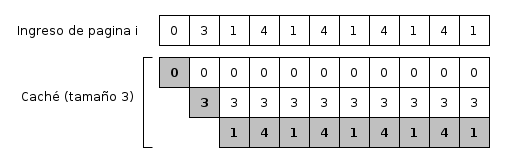
\includegraphics[scale=0.65]{diagramas/MRUPathological.png}\\
	\end{center}

\subsection{ Peor caso LRU: Traza LRUPathological} 
	En la siguiente traza para LRU, se intenta maximizar la cantidad de \textit{Miss} para el algoritmo. El patr\'on para lograrlo se basa
en completar la cach\'e con una traza y luego repetirla varias veces de forma de desalojar las mismas p\'aginas que se mantuvieron al principio.
Al completar la cach\'e se refencia una p\'agina nueva no existente, en el ejemplo la p\'agina 3, se desaloja la p\'agina m\'as antigua, la 0, que 
justamente es la siguiente a ser referenciada por la traza y que vendr\'a a desalojar a la p\'agina 1, que ser\'a justamente la siguiente en ser 
desalojada. De esta forma se ir\'an desalojando las p\'aginas que ser\'an inmediatamente referenciadas ocacionando una serie de \textit{Miss en cascada}. 

	\begin{center}
	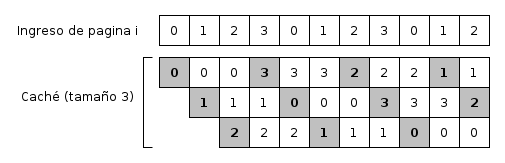
\includegraphics[scale=0.65]{diagramas/LRUPathological.png}\\
	\end{center}

\subsection{ LRU vs \textit{Touch Count}}

A continuaci\'on se describe un escenario en el cual el algoritmo de Touch Count mejora con respecto a LRU.

El ejemplo consiste en potenciar las p\'aginas que el Touch Count considera importantes, e intentar desalojarlas al mismo tiempo de la cach\'e en el
algoritmo LRU.\\

Inicialmente se utilizar\'a una traza cualquiera para completar la cach\'e. En ambos algoritmos estar inicializaci\'on dar\'a \textit{Miss} ya que
las p\'aginas no existir\'an.

Un escenario posible ser\'ia

\begin{itemize}
	\item[1)] full scan sobre la tabla A: para cargar las p'aginas en la cach\'e (se asume que los datos de A no superan el tama\~{n}o de la cach\'e.
	\item[2)] varios file scan sobre la tabla A condicionando a los registros con id par: en ambos algoritmos habr\'a \textit{Hit}.
	\item[3)] file scan sobre la tabla A condicionando a los registros con id impar: en ambos algoritmos habr\'a \textit{Hit}.
	\item[4)] file scan sobre la tabla B: en ambos algoritmos habr\'a \textit{Miss}.
	\item[5)] file scan sobre la tabla A: condicionando a los registros con id par: s\'olo en Touch Count las p\'aginas todav\'ia exisit\'ran en cach\'e.
ya que las reiteradas referncias del punto 2 habr\'an hecho que Touch Count les diera un pero mayor y por ende las habr\'ia salvado en la \textit{regi\'on caliente}.
\end{itemize}

La conclusi\'on que se intenta describir es que el Touch Count prioriza las p\'aginas por \textit{peso} mientras que LRU las prioriza por \'ultimo 
acceso.\\

Si una tabla tuvo sus p\'aginas accedidas recientemente, el algoritmo LRU tendr\'a sus p\'aginas como relevantes mientras que para Touch Count 
solo lo ser\'an si son refenciadas en m\'as ocaciones. \\

Por ello si una tabla fue accedida muchas veces, pero no \'ultimamente, 
posiblemente no sean tenida en cuenta por el algoritmo LRU mientras que Touch Count las tendr\'a como relevantes ya que tuvieron una frecuencia alta de
accesos. \\ 

En conclusi\'on Touch Count se basa en que si una p\'agina fue accedida muchas veces es probable que vuelva a ser referenciada, por eso les 
asigna un peso y pondera respecto a \'el. Por el contrario LRU se basa en que las p\'aginas m\'as recientes son las m\'as probables de volver a ser
referenciadas y son \'estas las que decide priorizar.

	\begin{center}
		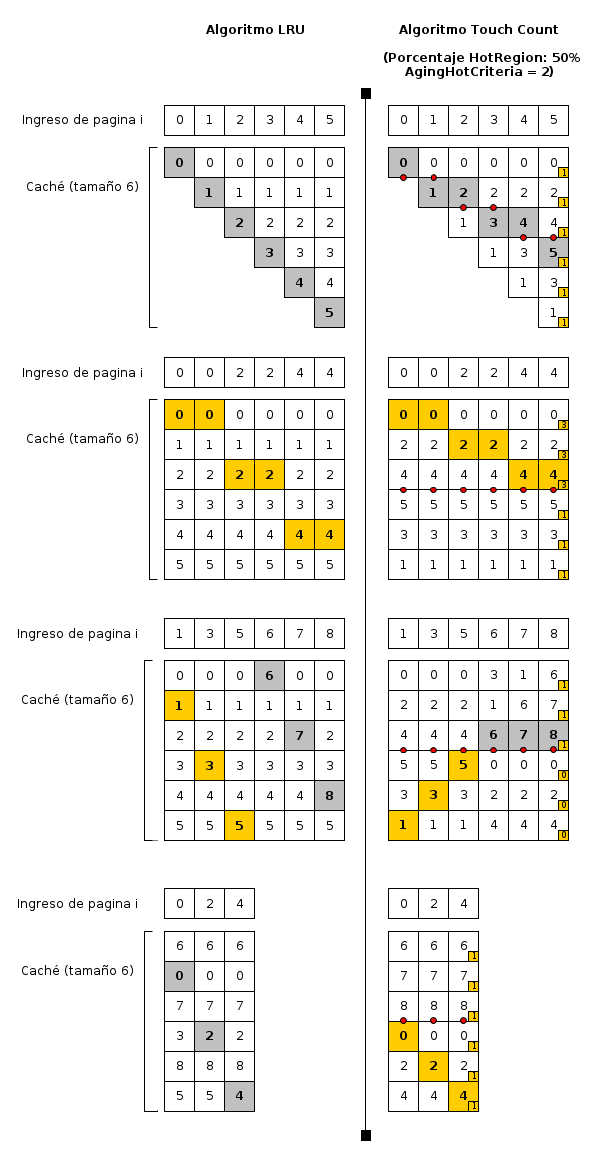
\includegraphics[scale=0.65]{diagramas/LRUvsTouchCountAll.png}\\
	\end{center}

	%\begin{center}
	%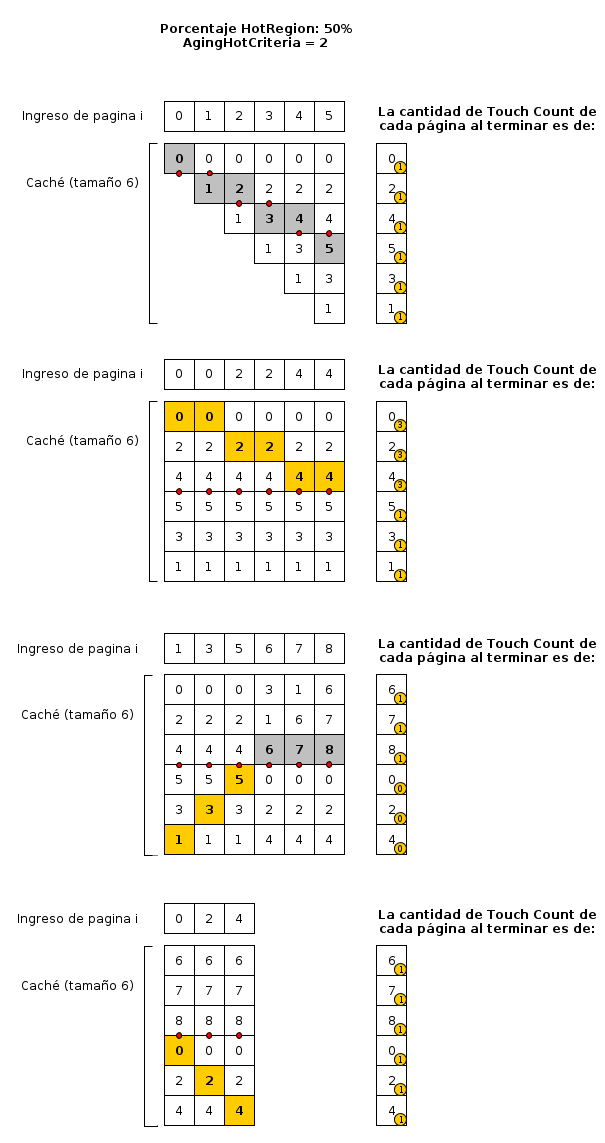
\includegraphics[scale=0.65]{diagramas/LRUvsTouchCount2.png}\\
	%\end{center}

\subsection{Traza: badMRUAndNotGodLRU}

Esta traza se gener\'o llevando al extremo las diferencias entre los algortimos.\\

Como vimos anteriormente el algoritmo de MRU no quita una p\'agina de la cach\'e hasta que esta no posea la referencia m\'as reciente. 
Inmediatamente se desprende que las p\'aginas que puedan llegar a la cach\'e y sean poco utilizadas tienen altas chances de evitar el desalojo.\\

El algoritmo de LRU si bien corrige el caso de MRU reci\'en mencionado, presenta como inconveniente que grandes pedidos de p\'aginas que producen
miss realizados de manera espor\'adica terminan barriendo la cach\'e, perdiendo p\'aginas que potencialmente pueden ser reutilizadas.\\

Touch count puede ser \'util para evitar ambos problemas: la parte fr\'ia act\'ua como una LRU, corrigiendo el problema de MRU. Por otro lado, 
da peso a las p\'aginas que son m\'as usadas evitando que por ejemplo, los file scans grandes las terminen por excluir de la cach\'e.\\

De esta manera y utilizando una cach\'e de 200 p\'aginas, se realizaron 7800 pedidos de la siguiente manera:\\

\begin{itemize}
    
	\item{Se llena la cach\'e y se vuelve a pedir cada p\'agina de la cach\'e tres veces (generando 200 miss y 600 hits).
Estas p\'aginas no vuelven a ser pedidas y al no pedir una misma p\'agina dos veces consecutivas, la cantidad de hits final m\'axima para MRU
ser\'a de 600.}\\

    \item{Se crea un ciclo donde la cach\'e se llena con p\'aginas siempre nuevas, provocando que LRU realice un flush completo. 
A su vez se referencia a un conjunto (fijo y distinto de todas las anteriores) de 50 p\'aginas (25\% de la cach\'e) agingHotCriteria + 1 veces, 
con el objeto de mantener en cach\'e en el algoritmo de \textit{Touch Count}.}\\ 

\end{itemize}

La traza se corre con el algoritmo de MRU, LRU y \textit{Touch Count}, este \'ultimo aceptando r\'afagas (para simplificar el problema) y 
con cuatro porcentajes de hot region (25\%, 50\%, 75\%, 90\%).\\

A continuaci\'on se detallan los resultados obtenidos.\\

\newpage

\begin{multicols}{2}
\noindent{\textbf{MRU}}\\
\textbf{Hits}: 600\\
\textbf{Misses}: 7200\\
\textbf{Hit rate}: 0.0769\\

\noindent{\textbf{TouchCount}} (25\% HOT)\\
\textbf{Hits:} 3550\\
\textbf{Misses:} 4250\\
\textbf{Hit rate:} 0.455\\

\noindent{\textbf{TouchCount}} (75\% HOT)\\
\textbf{Hits}: 3550\\
\textbf{Misses}: 4250\\
\textbf{Hit rate}: 0.455\\

\noindent{\textbf{LRU}}\\
\textbf{Hits:} 2971\\
\textbf{Misses:} 4829\\
\textbf{Hit rate:} 0.380\\

\noindent{\textbf{TouchCount}} (50\% HOT)\\
\textbf{Hits}: 3550\\
\textbf{Misses}: 4250\\
\textbf{Hit rate}: 0.455\\

\noindent{\textbf{TouchCount}} (90\% HOT)\\
\textbf{Hits}: 600\\
\textbf{Misses}: 7200\\
\textbf{Hit rate}: 0.0769\\

\end{multicols}


El rendimiento del algoritmo de MRU queda muy por debajo de los otros dos debido a que almacen\'o paginas que no volvieron a ser referenciadas
 como se explic\'o anteriormente.\\

El algoritmo de \textit{Touch Count} gana m\'as de un 7\% de mejora, al poder mantener ese conjunto de 50 p\'aginas a\'un cuando se efect\'ua 
el file scan.\\

Es muy interesante notar que no existe mejora de performance entre las variantes de \textit{Touch Count} de 25\%, contra las de  50\% y 75\% de
hot region. Esto es debe a que las p\'aginas que son continuamente referenciadas ocupan el 25\% de la cach\'e y nunca bajan a la cold region; 
adem\'as, como nada de la cold region sube (exceptu\'ando las del 25\%), el espacio entre el mid point marker y 
la primer p\'agina que se referencia continuamente queda con la carga inicial (utilizada para MRU) que al no ser vuelta a referenciar,
 no a\~{n}ade hits.\\

Por otro lado, cuando se utiliza el porcentaje de hot region en 90\%, se obtienen los mismos resultados que en MRU. Como ya mencionamos, 
los elementos son insertados como \'ultimo elemento de la cold region. La parte fr\'ia funciona como una LRU. 
Tenemos entonces una lista de tama\~{n}o 20 (10\% de la cach\'e) en la cual en una r\'afaga le agregamos 50 elementos. 
Luego de la carga, quedan los 20 \'ultimos y en la siguiente iteraci\'on cuando queremos referenciarlos, para aumentar el
 touch count en el mismo orden, poseemos el mismo problema que en LRU, nunca obtenemos un hit.\\

Se desprende necesariamente que el tama\~{n}o \'optimo de la hot region depende del tipo de carga que el servidor posee.
 Adem\'as, tener una zona fr\'ia muy chica fuerza a que para poder una p\'agina pasar a la zona caliente debe ser referenciada 
en una gran cantidad en poco tiempo y/o no pueden generarse gran cantidad de miss en cach\'e ya que forzar\'ian a que la
 p\'agina sea desalojada. Por otro lado, cuando m\'as chica es la zona c\'alida, mayor es la cantidad de llamadas 
que reciben las p\'aginas que posee, ya que si no son r\'apidamente desalojadas.\\

No se considera en la traza el par\'ametro de cantidad m\'axima de hits por segundo. 
Esto no significa que el tama\~{n}o \'optimo de la hot region sea independiente de \'el, as\'i como de la carga del servidor.
Evitar las r\'afagas dificulta mucho m\'as que una p\'agina pueda mantenerse en cach\'e, agregando un factor de periodicidad,
 es decir; no alcanza con haber sido requerida muchas veces en poco tiempo, peri\'odicamente debe ser llamada para evitar el desalojo.\\

Es v\'alido notar que tener igual hit rate con distinto porcentaje de hot region es un caso pr\'acticamente exclusivo de nuestra carga de datos.
 Al tener una mayor cantidad de p\'aginas salvadas en la zona c\'alida, existe mayor probabilidad que se referencie alguna de ellas una nueva vez
 (excluyendo los casos extremos considerados en el p\'arrafo anterior).\\

A continuaci\'on veremos un test en donde los porcentajes difieren.\\

\newpage
\subsection{Traza: smallQueriesAndOneBigFileScan}


Se cre\'o una nueva traza con el objeto de analizar qu\'e sucede cuando existen pedidos de sets peque\~{n}os de datos de manera 
peri\'odica y se produce un pedido grande que supera el tama\~{n}o de la cach\'e de p\'aginas, 
las cuales todas producen miss, en nuestro caso emulado con un file scan.\\

Para ellos se generaran cinco conjuntos de p\'aginas:

\begin{itemize}
    \item{P\'aginas de la tabla \textit{music} (tama\~{n}o 5\% de la cach\'e).}
    \item{P\'aginas de la tabla \textit{artist} (tama\~{n}o 5\% de la cach\'e).}
    \item{P\'aginas de la tabla \textit{label} (tama\~{n}o 15\% de la cach\'e).}
    \item{P\'aginas aleat\'oreas en cada iteraci\'on de la tabla \textit{countrysales} (tama\~{n}o 3\% de la cach\'e).}
    \item{P\'aginas de la tabla \textit{g\'enero} (tama\~{n}o 2 * (tama\~{n}o de cache + offset)).}
\end{itemize}

En cada iteraci\'on, se generan p\'aginas aleat\'oreas para la tabla countrysales y se piden todas las p\'aginas menos la de genre
(ya que estas se corresponden con nuestro \textit{big file scan}).
 Cabe destacar, que con el objeto de no condicionar el resultado, el orden en la que se encolan los pedidos 
de p\'aginas de cada tabla es randomizado. 
En la mitad de las iteraciones, se pide el file scan de g\'enero\\

Se permitieron por simplicidad de la traza, r\'afagas. El par\'ametro agingHotCriteria es de 10 y el tama\~{n}o de cach\'e es de 400.\\
La traza consta de 8272 pedidos de p\'aginas y los resultados obtenidos fueron:
   
\begin{multicols}{2}

\noindent{\textbf{MRU}}\\
\textbf{Hits: 6613}\\
\textbf{Misses: 1659}\\
\textbf{Hit rate: 0.799}\\

\noindent{\textbf{LRU}}\\
\textbf{Hits: 6692}\\
\textbf{Misses: 1580}\\
\textbf{Hit rate: 0.808}\\

\noindent{\textbf{TouchCount}} (25\% HOT)\\
\textbf{Hits: 6792}\\
\textbf{Misses: 1480}\\
\textbf{Hit rate: 0.821}\\

\noindent{\textbf{TouchCount}} (50\% HOT)\\
\textbf{Hits: 6849}\\
\textbf{Misses: 1423}\\
\textbf{Hit rate: 0.827}\\

\noindent{\textbf{TouchCount}} (75\% HOT)\\
\textbf{Hits: 6907}\\
\textbf{Misses: 1365}\\
\textbf{Hit rate: 0.834}\\

\noindent{\textbf{TouchCount}} (90\% HOT)\\
\textbf{Hits: 6902}\\
\textbf{Misses: 1370}\\
\textbf{Hit rate: 0.834}\\

\end{multicols}

El algoritmo MRU presenta mejor resultado al de la traza anterior. Esto se debe a que puede resolver el problema del file scan grande, 
como la p\'agina m\'as reciente es la que acaba de agregar (perteneciente adem\'as al \'unico pedido grande), la remueve y evita perder el 
resto de las p\'aginas perteneciente a las \textit{small queries} que son las que generan hits.\\

La diferencia de performance entre MRU y LRU se debe al pedido de las p\'aginas aleatorias de countrysales. 
Por como est\'a implementado el algoritmo, el pedido de estas p\'aginas se realiza en un entorno temporal cercano 
al pedido del resto de las consultas peque\~{n}as. Si la cach\'e se encuentra llena, como sucede luego del file scan, 
MRU tendr\'a a desalojar a p\'aginas de las consultas peque\~{n}as que luego generar\'an miss, en cambio LRU y a medida
que pasen los pedidos, tendr\'a a remover las p\'aginas procedentes al file scan.\\

No es menor la mejora que genera el algoritmo de \textit{Touch Count} en compaci\'on con LRU y MRU. 
Al poseer un 25\% de p\'aginas que se frecuentan y un 3\% de p\'aginas random que se van agregando, 
de las cuales posiblemente se repitan en el tiempo; estas se salvan en la zona caliente y el file scan no provoca su desalojo.\\

Se puede inferir que a medida que el porcentaje de zona caliente aumenta, la mejora del hit rate se va estabilizando. 
Nuevamente esto depende de la carga a la que se est\'e sometiendo al motor de base de datos.
 Para este ejemplo en particular, parecer\'ia sensato tomar como hot region alg\'un valor entre 25\% y 50\% 
y dejar el resto de la cach\'e como zona fr\'ia suponiendo que la carga continuara de similar manera y dejando espacio tanto en caliente como fr\'io para alg\'un caso at\'ipico que pueda suceder.

\section{C\'odigo fuente}

\section{Referencias}

\end{document}
